\documentclass{article}
\usepackage{amsmath}
\usepackage{graphicx}
\title{\bf{Manufactured Solution for the Incompressible Navier-Stokes}}
\author{Nicholas Malaya \\ Robert D. Moser} \date{}

\begin{document}
\maketitle

Construct a 3D incompressible field. Define three functions: f(x), g(y),
h(z) satisfying boundary conditions. 

Define the three components of velocity as,
\begin{align}
u = a f(x)  g'(y)  h'(z) \\
v = b f'(x) g(y)   h'(z) \\
w = c f'(x) g'(y)  h(z) 
\end{align}
To satisfy continuity, $a+b+c=0$. We can include time dependence
$a=a(t)$ if we so desire.

To ensure that the wall-normal velocity, v, is  zero at the walls ($y=-1,1$), choose
g(y) such that, 
\begin{equation}
 g(y) = (1-y^2)^2 \tilde g(y)
\end{equation}
Let's pick $\tilde g(y)$ to be,
\begin{equation}
\tilde g(y) = (y^5 + y^4 + y^3 + y^2 + y)
\end{equation}
An example of the full g(y) is shown in fig. \ref{gy}.

\begin{figure}
 \centering
 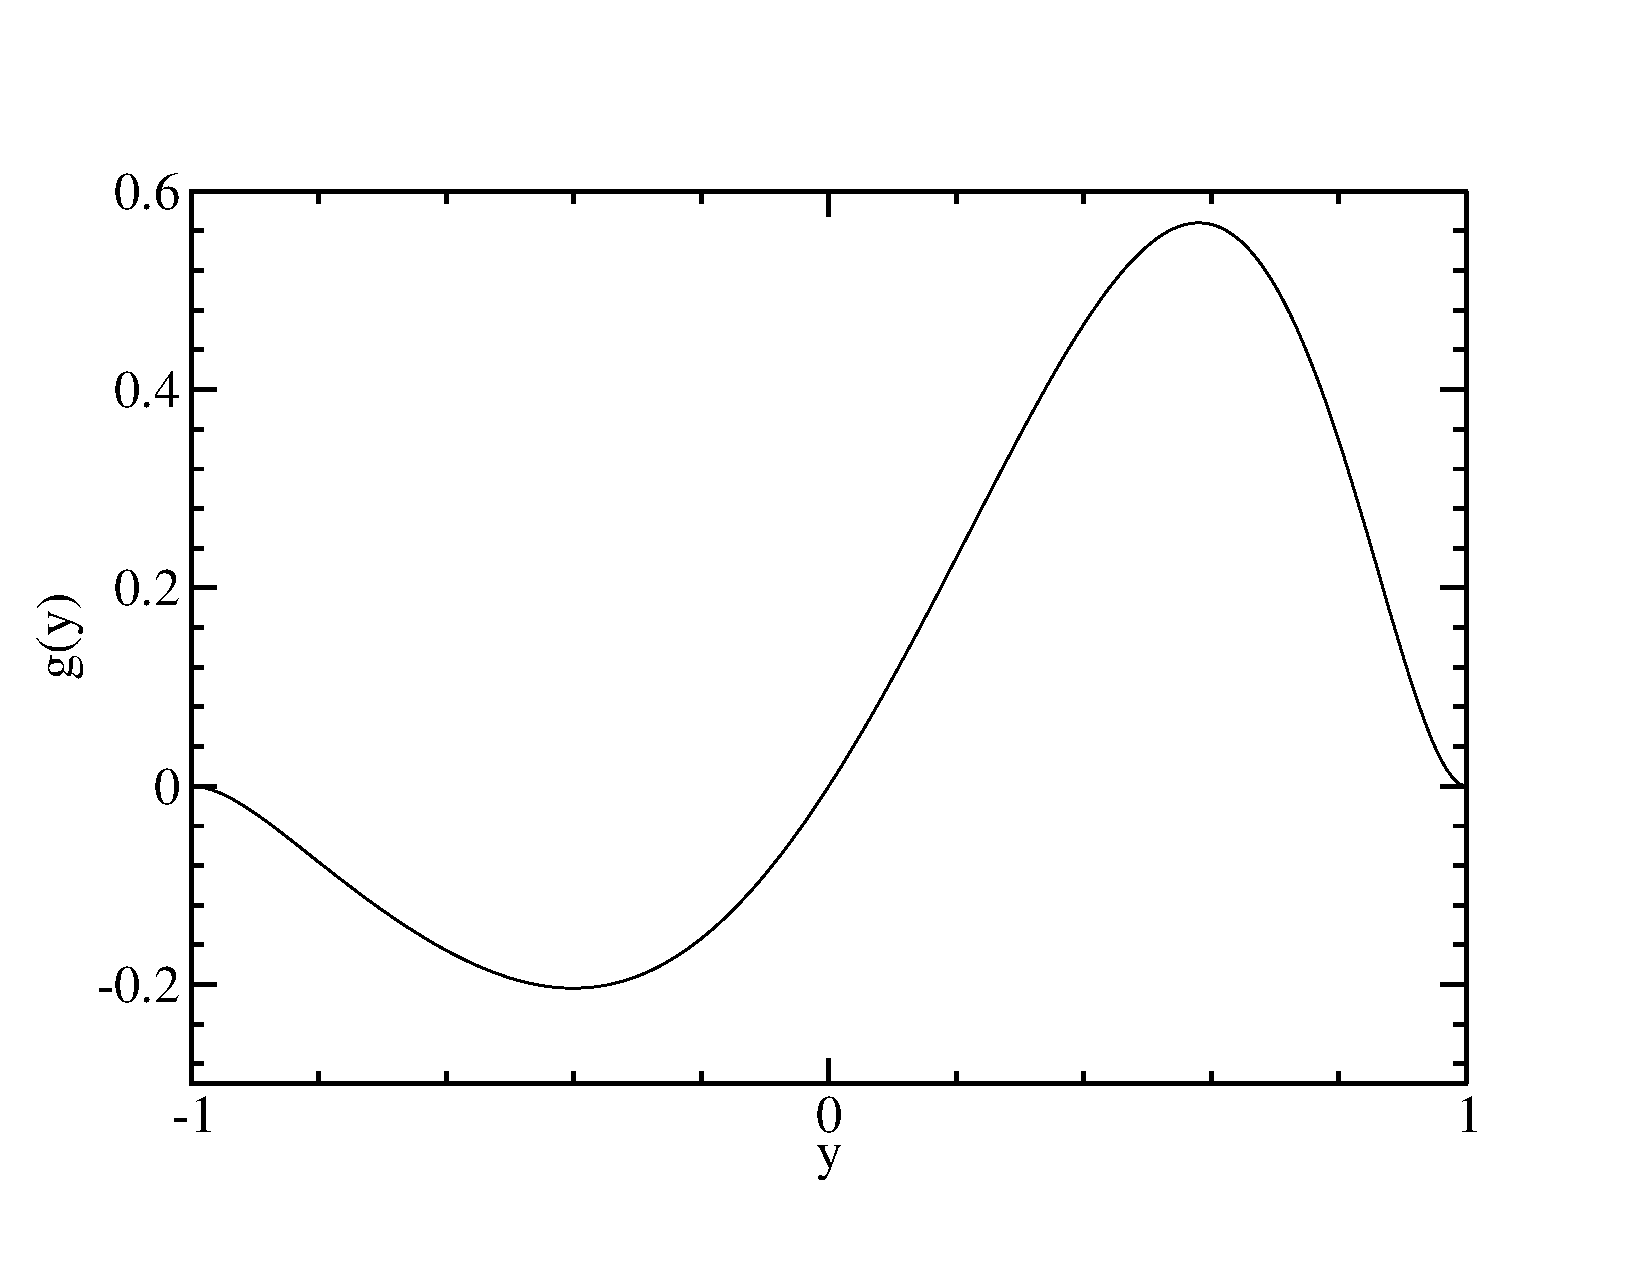
\includegraphics[width=0.5\textwidth]{gtilde.pdf}
 %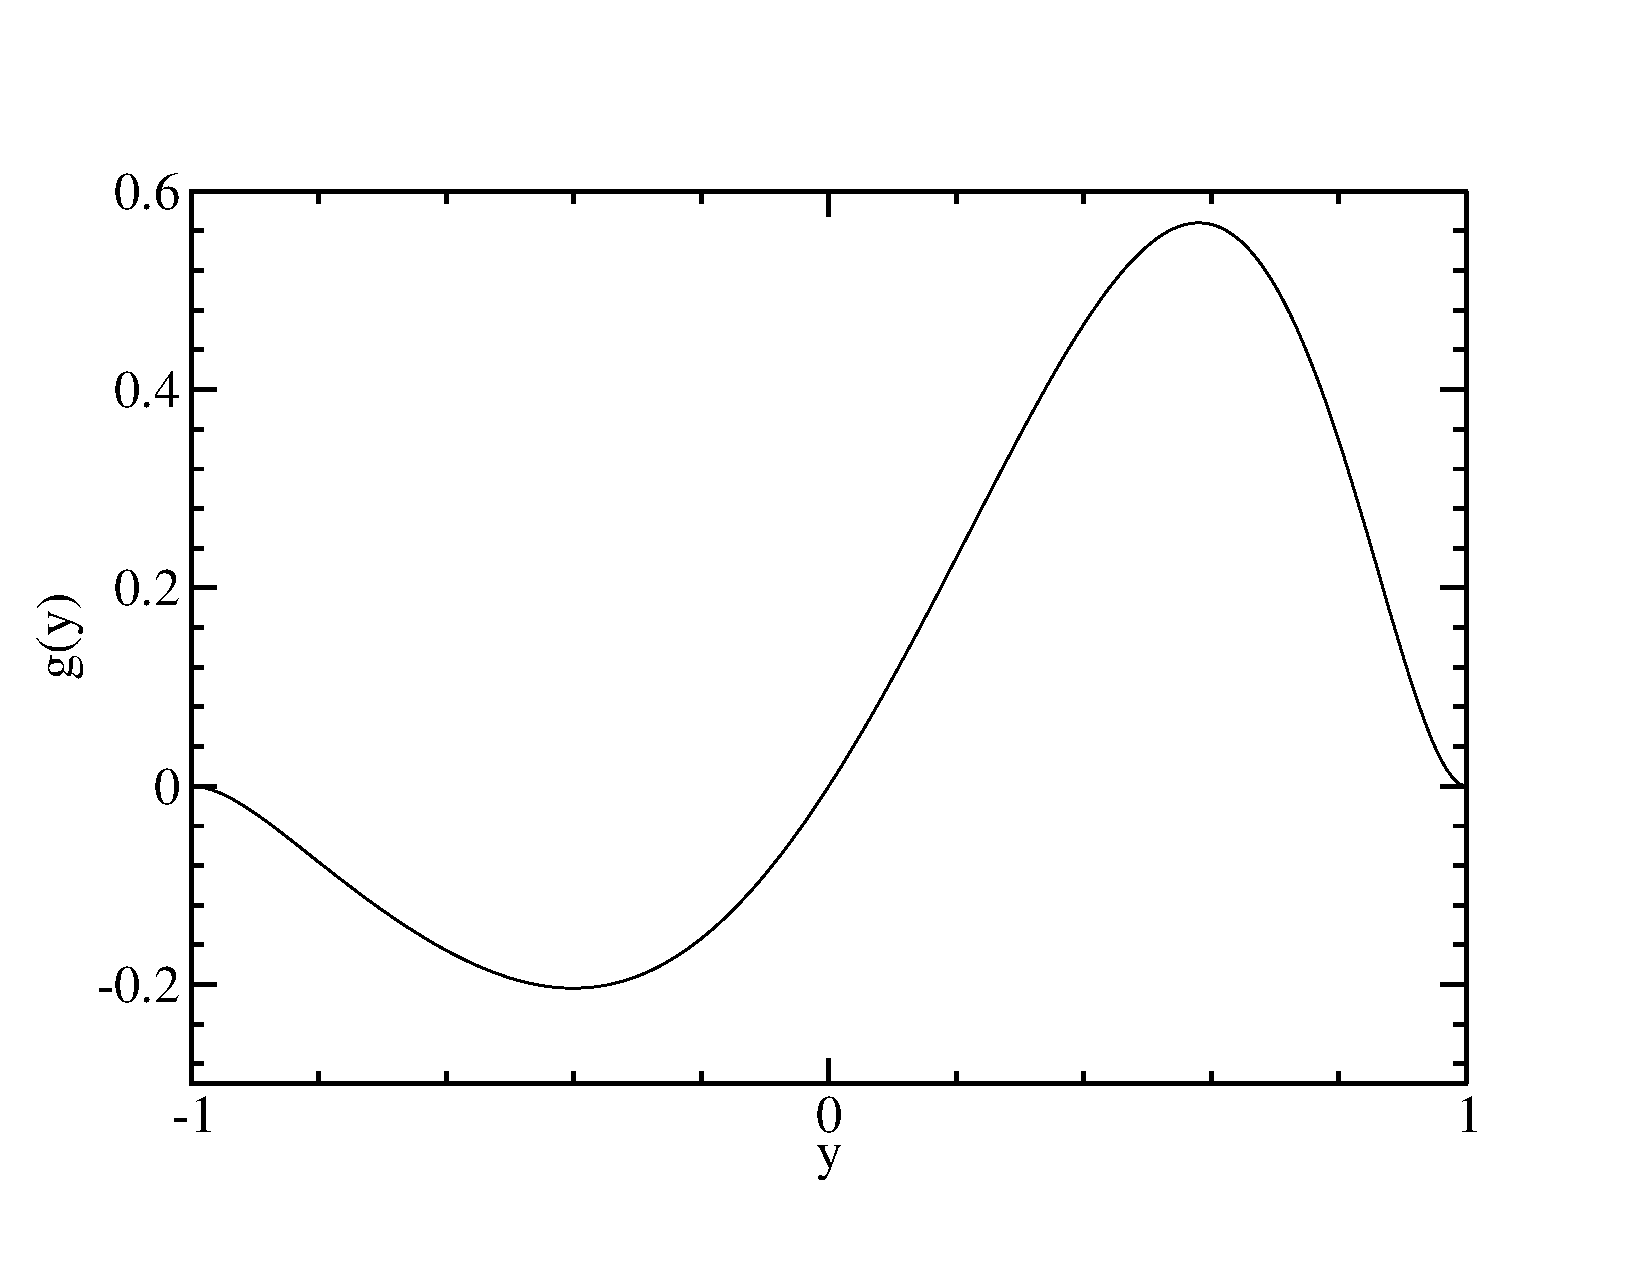
\epsfig{file=gtilde.pdf, height=1.7in,clip=}
 \caption{The manufactured solution, g(y)}
 \label{gy}
\end{figure}


In order to provide high wavenumber content, choose f(x) as,
\begin{equation}
 f(x) =
  \begin{cases}
   \text{sin}(k_x x)  \\
   \frac{1}{\beta + \text{sin}(k_x x)} & \mbox{if } \beta > 1 \\
  \end{cases}
\end{equation}
Likewise choose the manufactured solution for the spanwise component of
velocity to be
\begin{equation}
 h(z) =
  \begin{cases}
   \text{sin}(k_z z)  \\
   \frac{1}{\gamma + \text{sin}(k_z z)} & \mbox{if } \gamma > 1 \\
  \end{cases}
\end{equation}
Finally, manufacture the pressure such that, 
\begin{equation}
 P = d f(x) \tilde g(y) h(z)
\end{equation}


\end{document}